\Exercise[number={2}]
A variable \(x\) in \(\mathbf{R}^2\) is emitted by two possible sources,
\(w_1\) and \(w_2\), of probability \(Pr(w_1)=p\) and \(Pr(w_2)=1-p\). 
We intend to design a Bayes classifier that assigns the correct class to each
observed \(x\). If the \(p(x|w_i)\) both have a Gaussian distribution, with
mean \(\mu_i\) and variance \(I\sigma^2\) (same for the two classes),
draw the boundaries of the decision regions as \(p\) varies.

\Answer[number={2}]
The boundaries of a binary classifier can be studied by computing the
sign of \(z(x)\), with \(z\) being the exponent of the sigmoid function, in
particular the decision boundaries are given by \(z(x)=0\).
\begin{align*}
    z(x)
    &=\log{\frac{p(x|w_1)}{p(x|w_2)}} + \log{\frac{Pr(w_1)}{Pr(w_2)}}
    =\log{p(x|w_1)}-\log{p(x|w_2)}+\log{\frac{p}{1-p}}\\
    &=-\cancel{\log{\frac{2\pi}{2\pi}}}-\cancel{\frac{1}{2}\log{\frac{|\Sigma_1|}{|\Sigma_2|}}}-\frac{1}{2\sigma^2}\bigl[(x-\mu_1)^T(x-\mu_1)-(x-\mu_2)^T(x-\mu_2)\bigr]+\log{\frac{p}{1-p}}\\
    &=-\frac{1}{2\sigma^2}\bigl[(\mu_1^T\mu_1-\mu_2^T\mu_2)-2(\mu_1-\mu_2)^Tx\bigr]+\log{\frac{p}{1-p}}\\
    &=-\frac{1}{2\sigma^2}\bigl[(\mu_1-\mu_2)^T(\mu_1+\mu_2-2x)\bigr]+\log{\frac{p}{1-p}}\\
    &=\frac{1}{\sigma^2}\biggl[(\mu_1-\mu_2)^T(x-\frac{\mu_1-\mu_2}{2})\biggr]+\log{\frac{p}{1-p}}
\end{align*}
\begin{align*}
    z(x)=0 \Longleftrightarrow \frac{1}{\sigma^2}\biggl[(\mu_1-\mu_2)^T(x-\frac{\mu_1-\mu_2}{2})\biggr]+\log{\frac{p}{1-p}}=0
\end{align*}
Notice that the first part of the equation is derived from
\(\log{\frac{p(x|w_1)}{p(x|w_2)}}\) and it must be zero on the decision
boundary, as both the likelihoods must be equal to 0.5. Moreover, it represents
a scalar product between two vectors: the first one represents the line
connecting \(\mu_1\) and \(\mu_2\), the second one is the line connecting
a generic \(x\) to the middle point of the line connecting the two means.
However, due to the presence of the right-side term \(\log{\frac{p}{1-p}}\),
the intersection point with the \(\mu_1-\mu_2\) line is moved from
the middle point towards the class center having a lower probability \(Pr(w_i)\),
making the area on the plane accounting for that lower probability class smaller.
In the 3D space, the equation \(z(x)=(\mu_1-\mu_2)^T(x-\frac{\mu_1-\mu_2}{2})\)
represents a hyperplane (in this case a plane), with an offset
\(\log{\frac{p}{1-p}}\), affecting where the plane intersects the plane
generated by \(x_1\) and \(x_2\) components.
Hence, three cases are possible:
\begin{enumerate}
    \item \(Pr(w_1)=Pr(w_2)=0.5\Rightarrow\log{\frac{p}{1-p}}=0\):
    the scalar product between the aforementioned vectors is null, implying
    that the two vectors must be perpendicular. Consequently, the following
    image, representing the decision boundaries, can be drawn:
    \begin{figure}[H]
        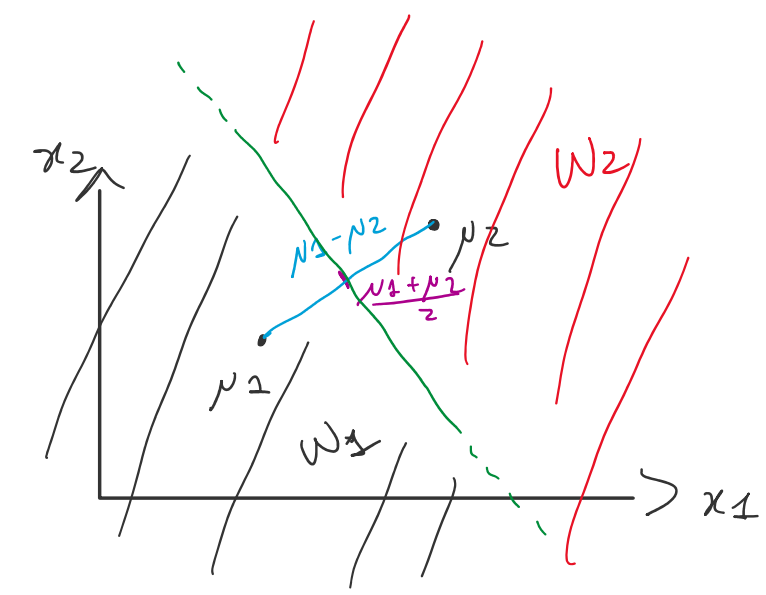
\includegraphics[scale=0.45]{C_2}
        \centering
    \end{figure}
    \item \(Pr(w_1)=p>Pr(w_2)=1-p\Rightarrow\log{\frac{p}{1-p}}>0\):
    the scalar product must once again be zero, however, the factor
    \(\log{\frac{p}{1-p}}\) implies a translation of the decision line
    toward the \(\mu_2\) mean. This is consistent with a translation
    toward the negative side of the sigmoid, since there is a bias
    toward the selection of class \(w_1\) (\(Pr(w_1)>0.5\)).
    \item \(Pr(w_1)=p<Pr(w_2)=1-p\Rightarrow\log{\frac{p}{1-p}}<0\):
    the scalar product must once again be zero, however, the factor
    \(\log{\frac{p}{1-p}}\) implies a translation of the decision line
    toward the \(\mu_1\) mean. This is consistent with a translation
    toward the positive side of the sigmoid, since there is a bias
    toward the selection of class \(w_2\) (\(Pr(w_2)>0.5\)).
  \end{enumerate}